\documentclass{scrartcl}
\usepackage{german}
\usepackage[T1]{fontenc}
\usepackage[latin1]{inputenc}
\usepackage[german]{babel}

% zusätzliche mathematische Symbole, AMS=American Mathematical Society
\usepackage{amssymb}

% fürs Einbinden von Graphiken
\usepackage{graphicx}

% für Namen etc. in Kopf- oder Fußzeile
\usepackage{fancyhdr}

% erlaubt benutzerdefinierte Kopfzeilen
\pagestyle{fancy}

% Definition der Kopfzeile
\lhead{
\begin{tabular}{ll}
Fisnik Zeqiri & 4306430 \\
Felix  Karg   & 4342014
\end{tabular}
}
\chead{}
\rhead{\today{}}
\lfoot{}
\cfoot{Seite \thepage}
\rfoot{}

\begin{document}
\section*{Antworten zum �bungsblatt Nr. 7}

\section*{Aufgabe 1}
        [Aufgabe 1] \\
	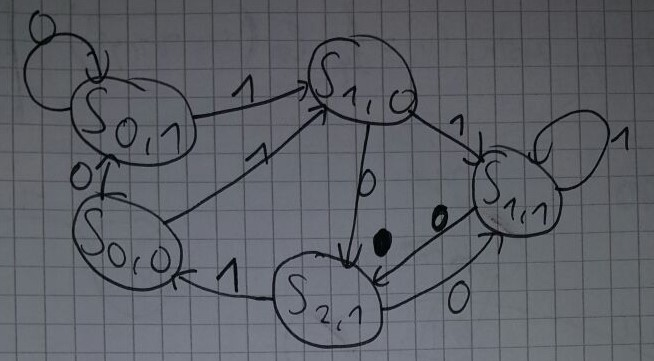
\includegraphics[width=16cm]{1.jpg}
\section*{Aufgabe 2}
        a) \\
        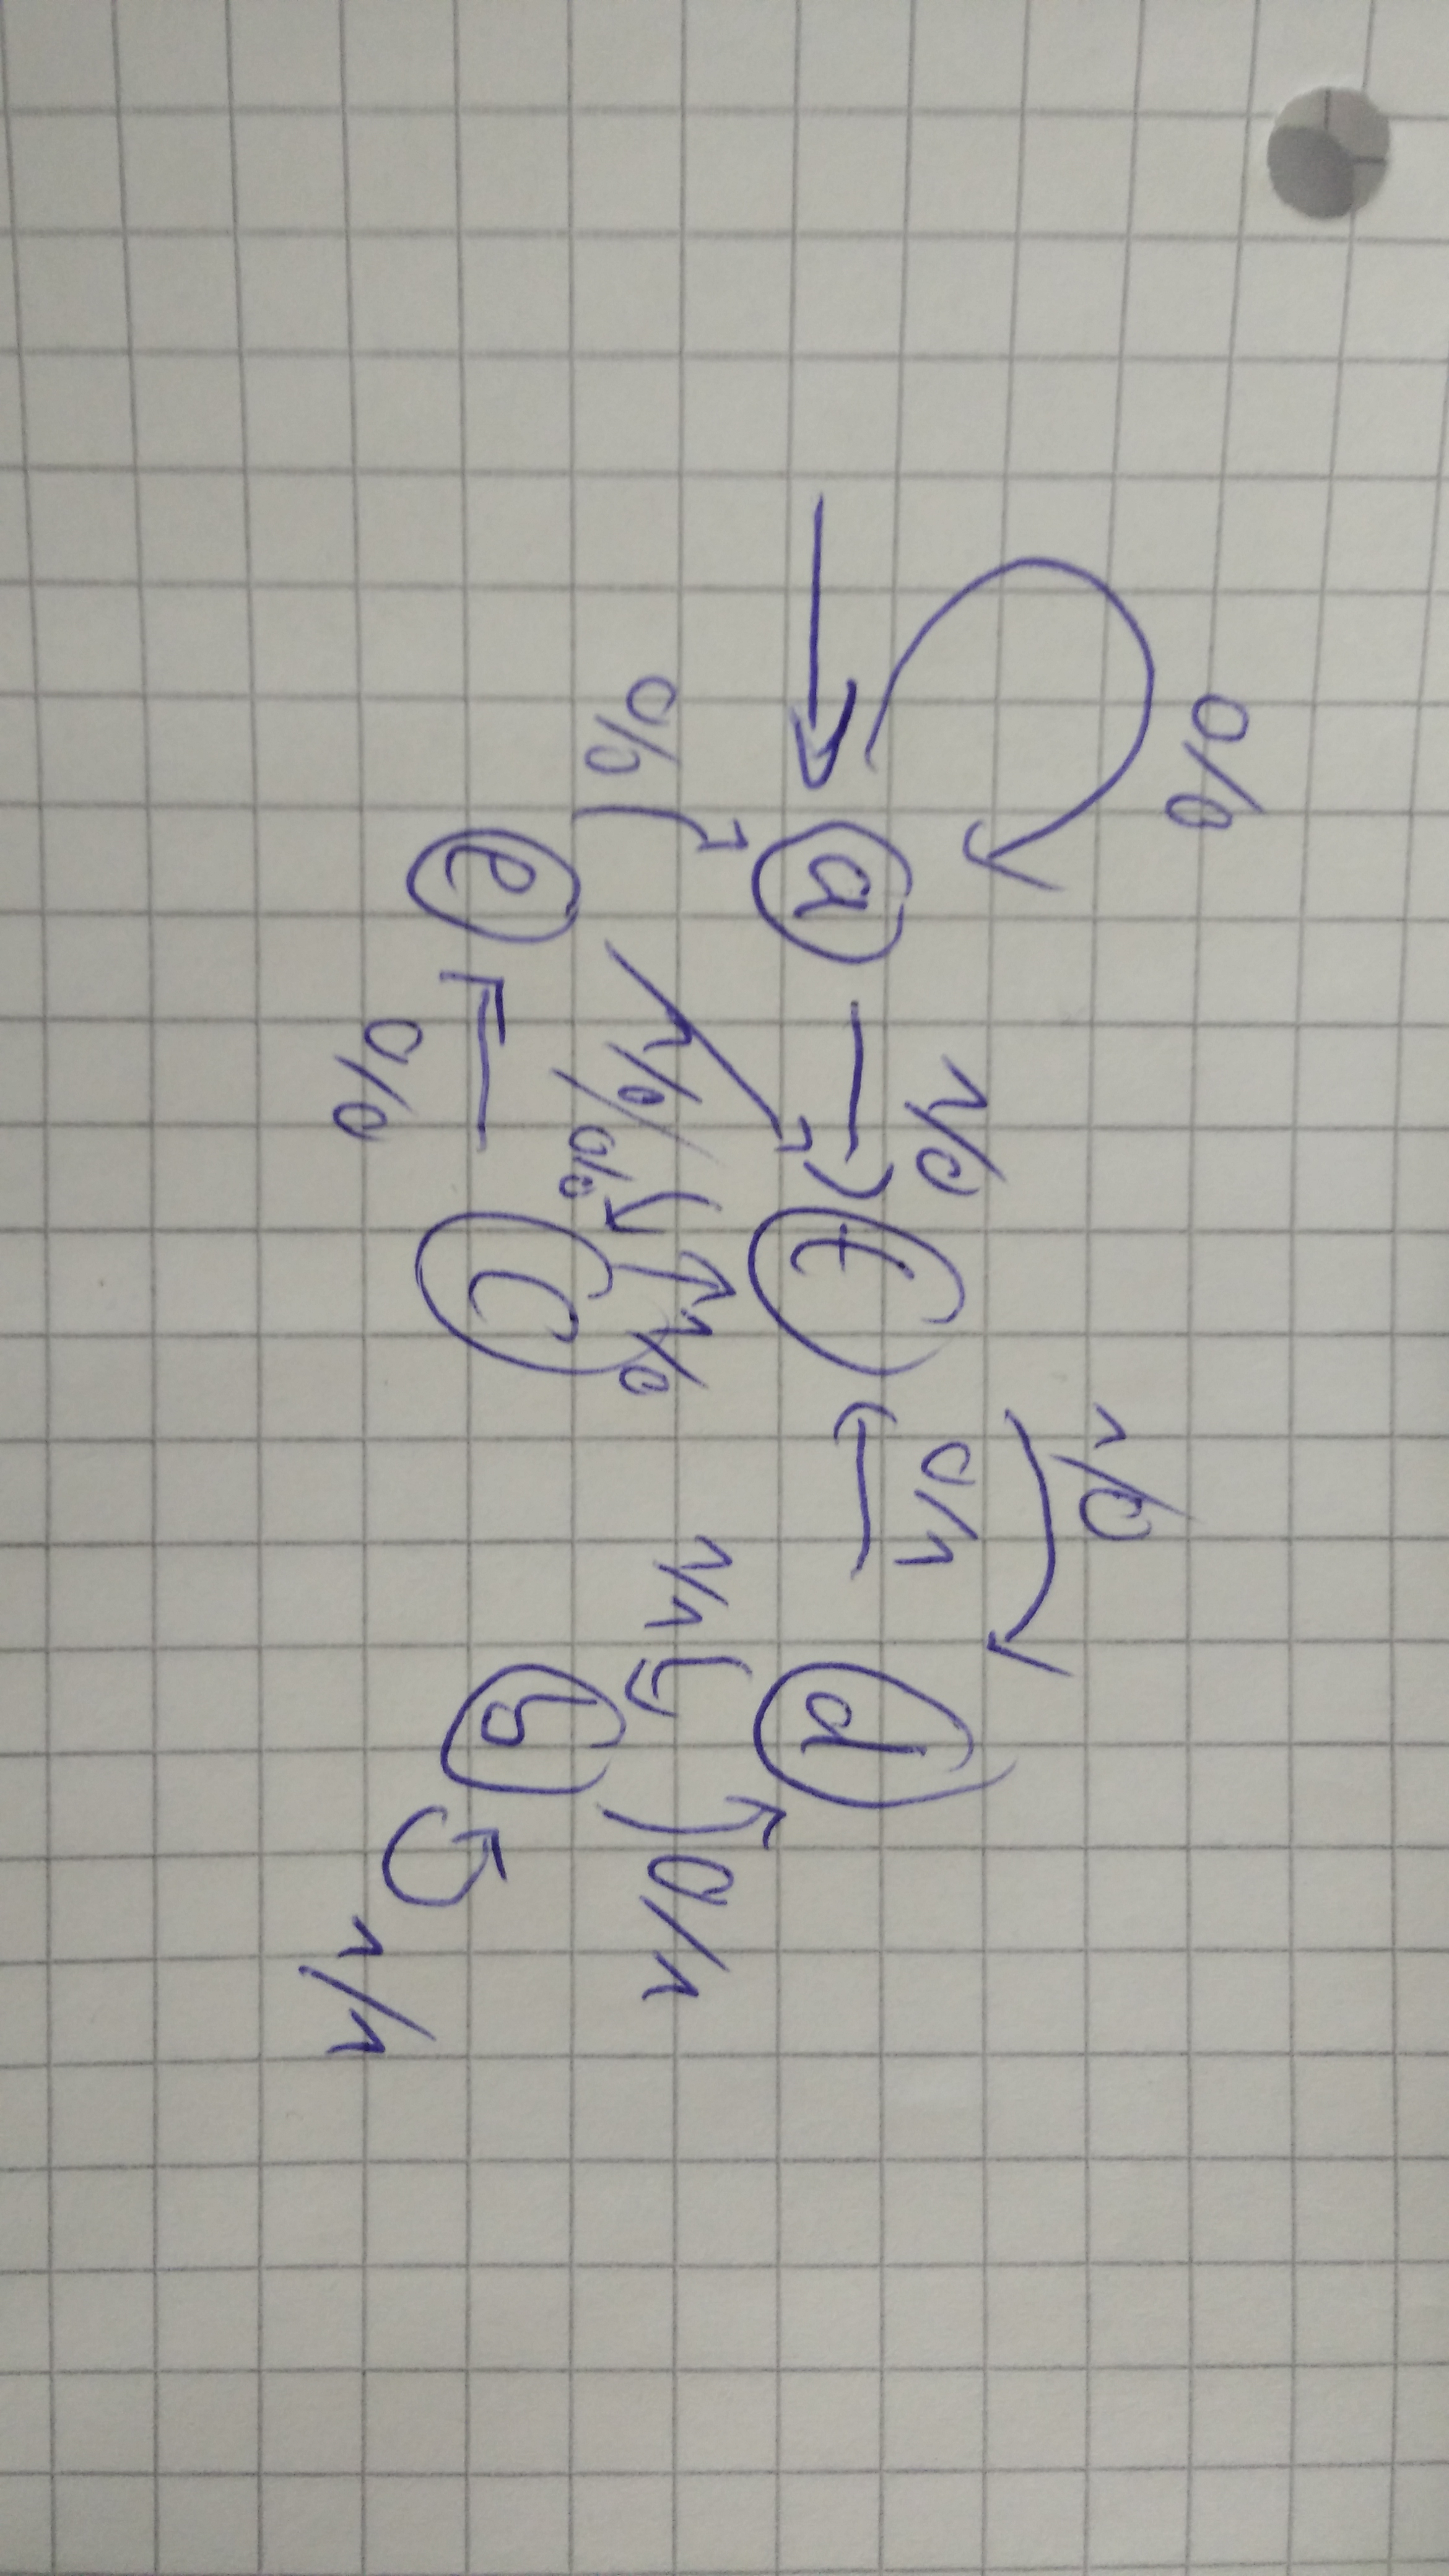
\includegraphics[width=12cm]{IMG_20161209_122056.jpg} \\
        Aufgabe 2 b) \\
	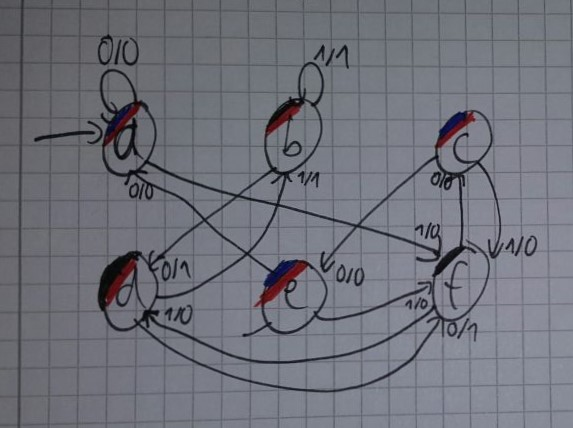
\includegraphics[width=13cm]{2a.jpg} \\
	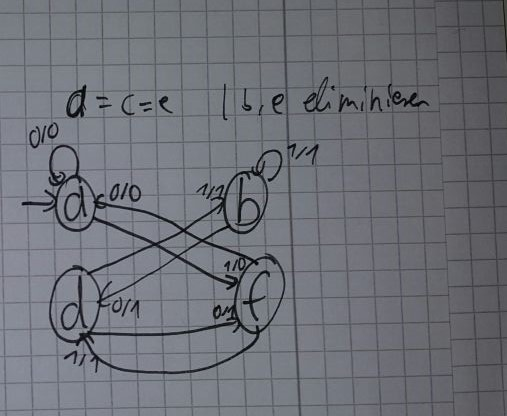
\includegraphics[width=13cm]{2b.jpg}
        Aufgabe 2 c) \\
	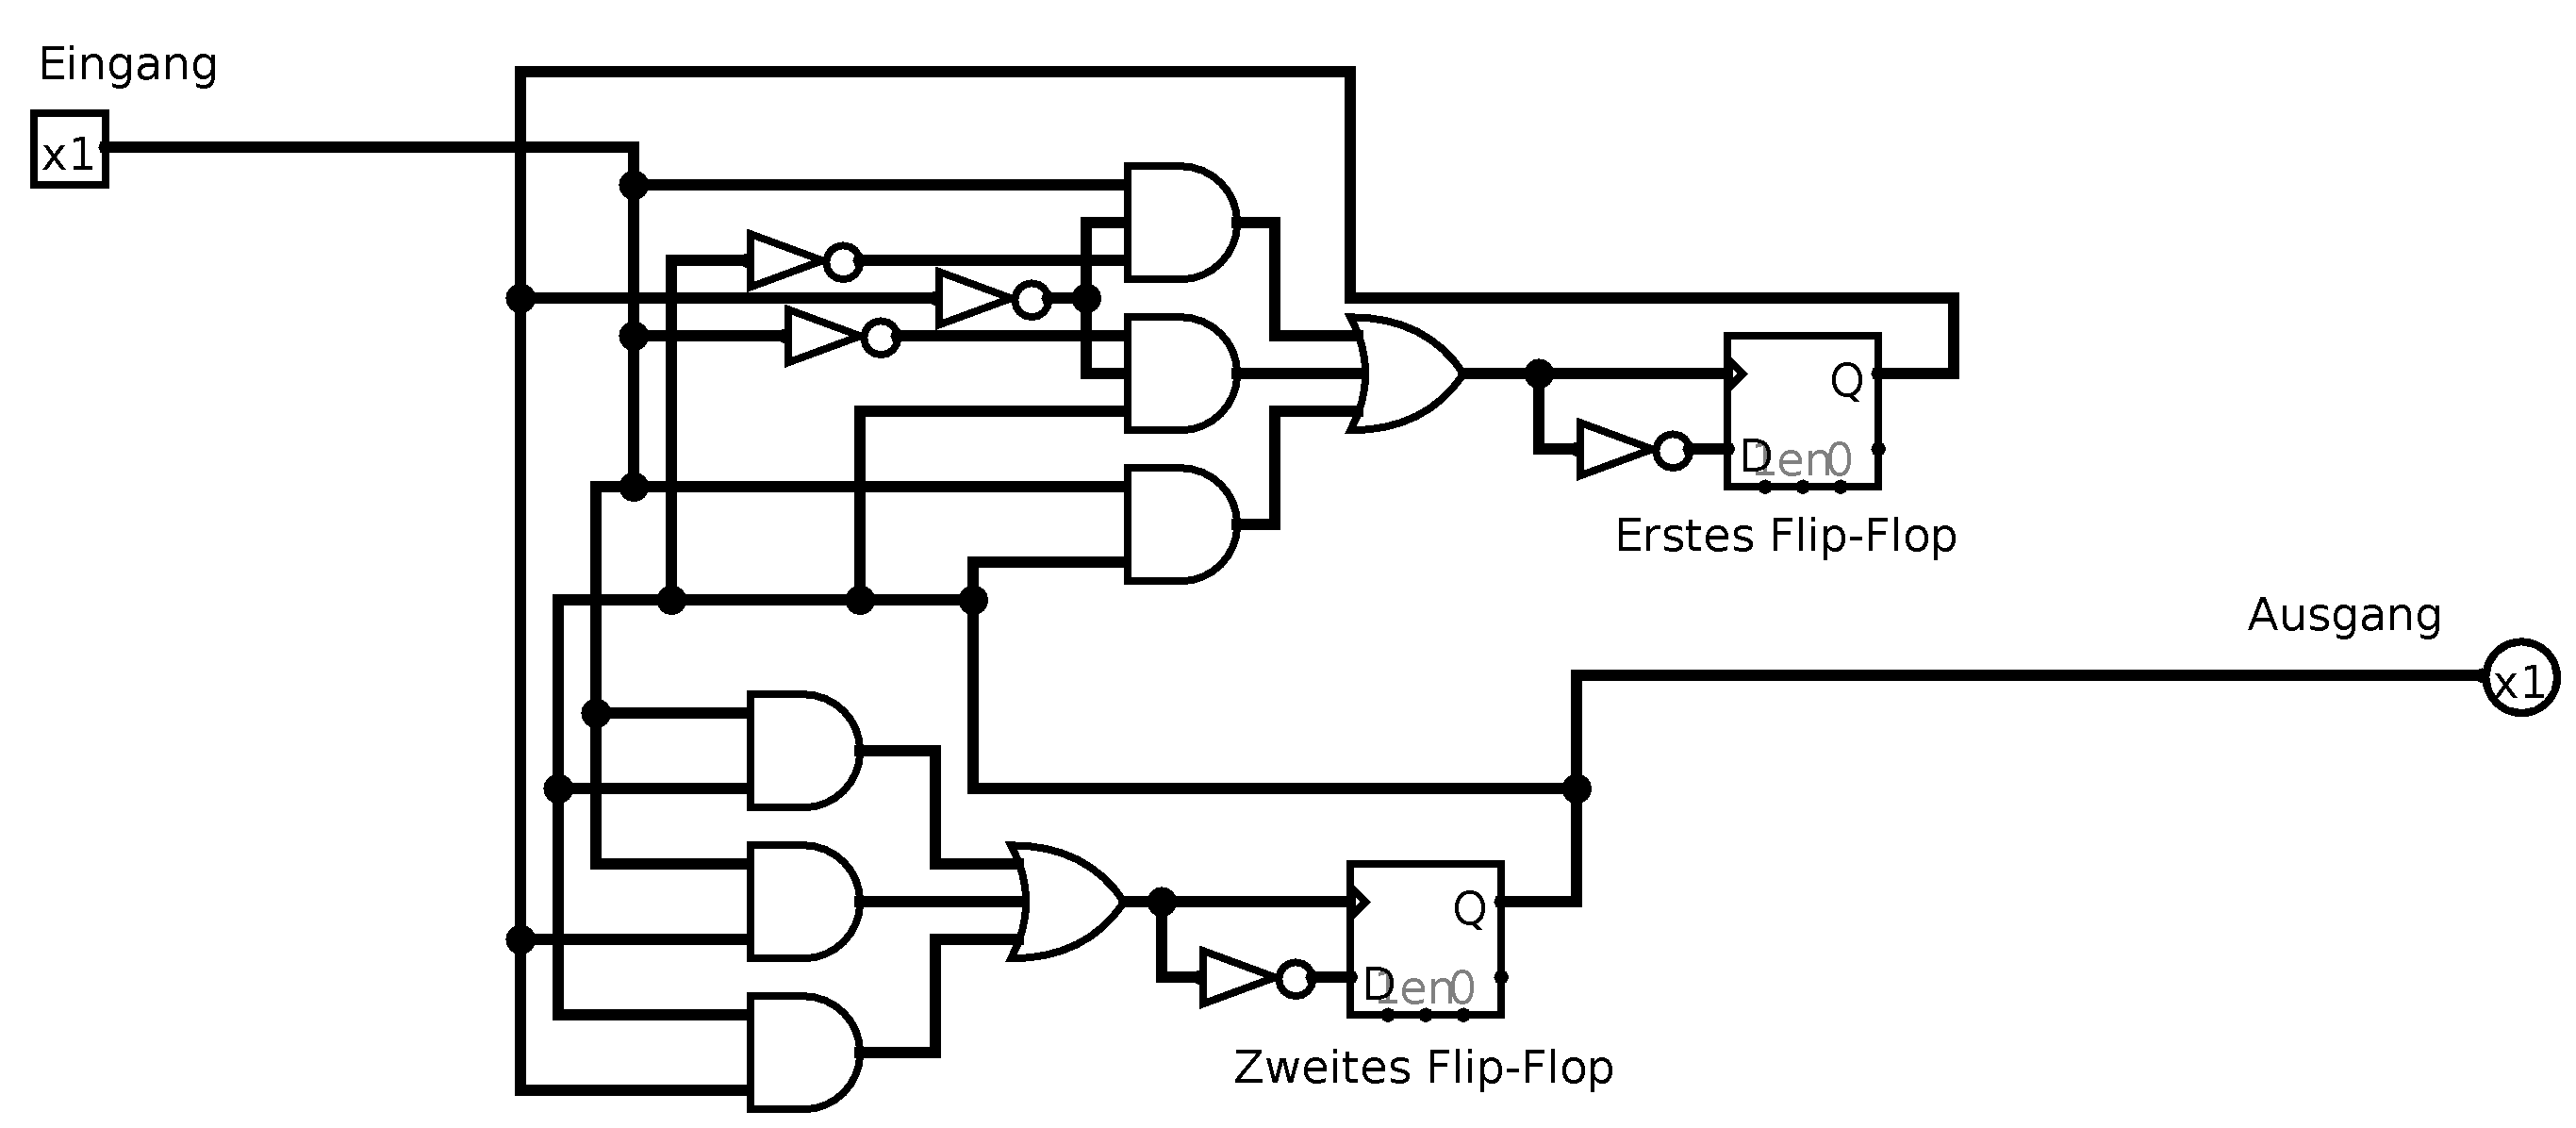
\includegraphics[width=13cm]{circuit_4.png} \\
        Bedingung ist, dass das neue Signal kommt, sobald die Flip-Flops
        jeweils geschalten haben. Der Anfangszustand (a) beider FF's ist 0.
        (Beide FF's sind active-High.)
\section*{Aufgabe 3}
\begin{itemize}
    \item[a)] [Schaltkreis 1] \\
	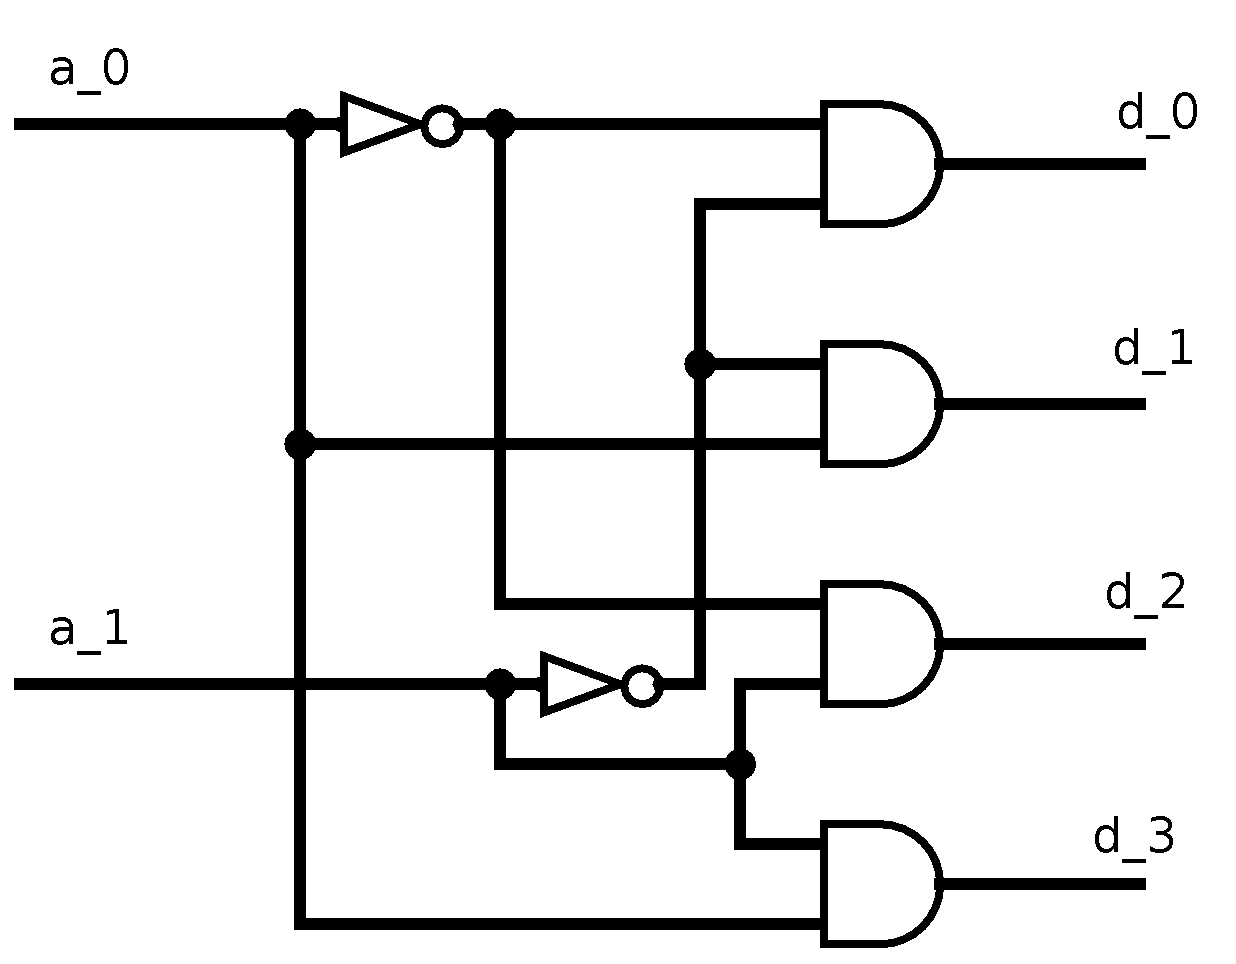
\includegraphics[width=13cm]{circuit_1.png}
    \item[b)] [Schaltkreis 2] \\
	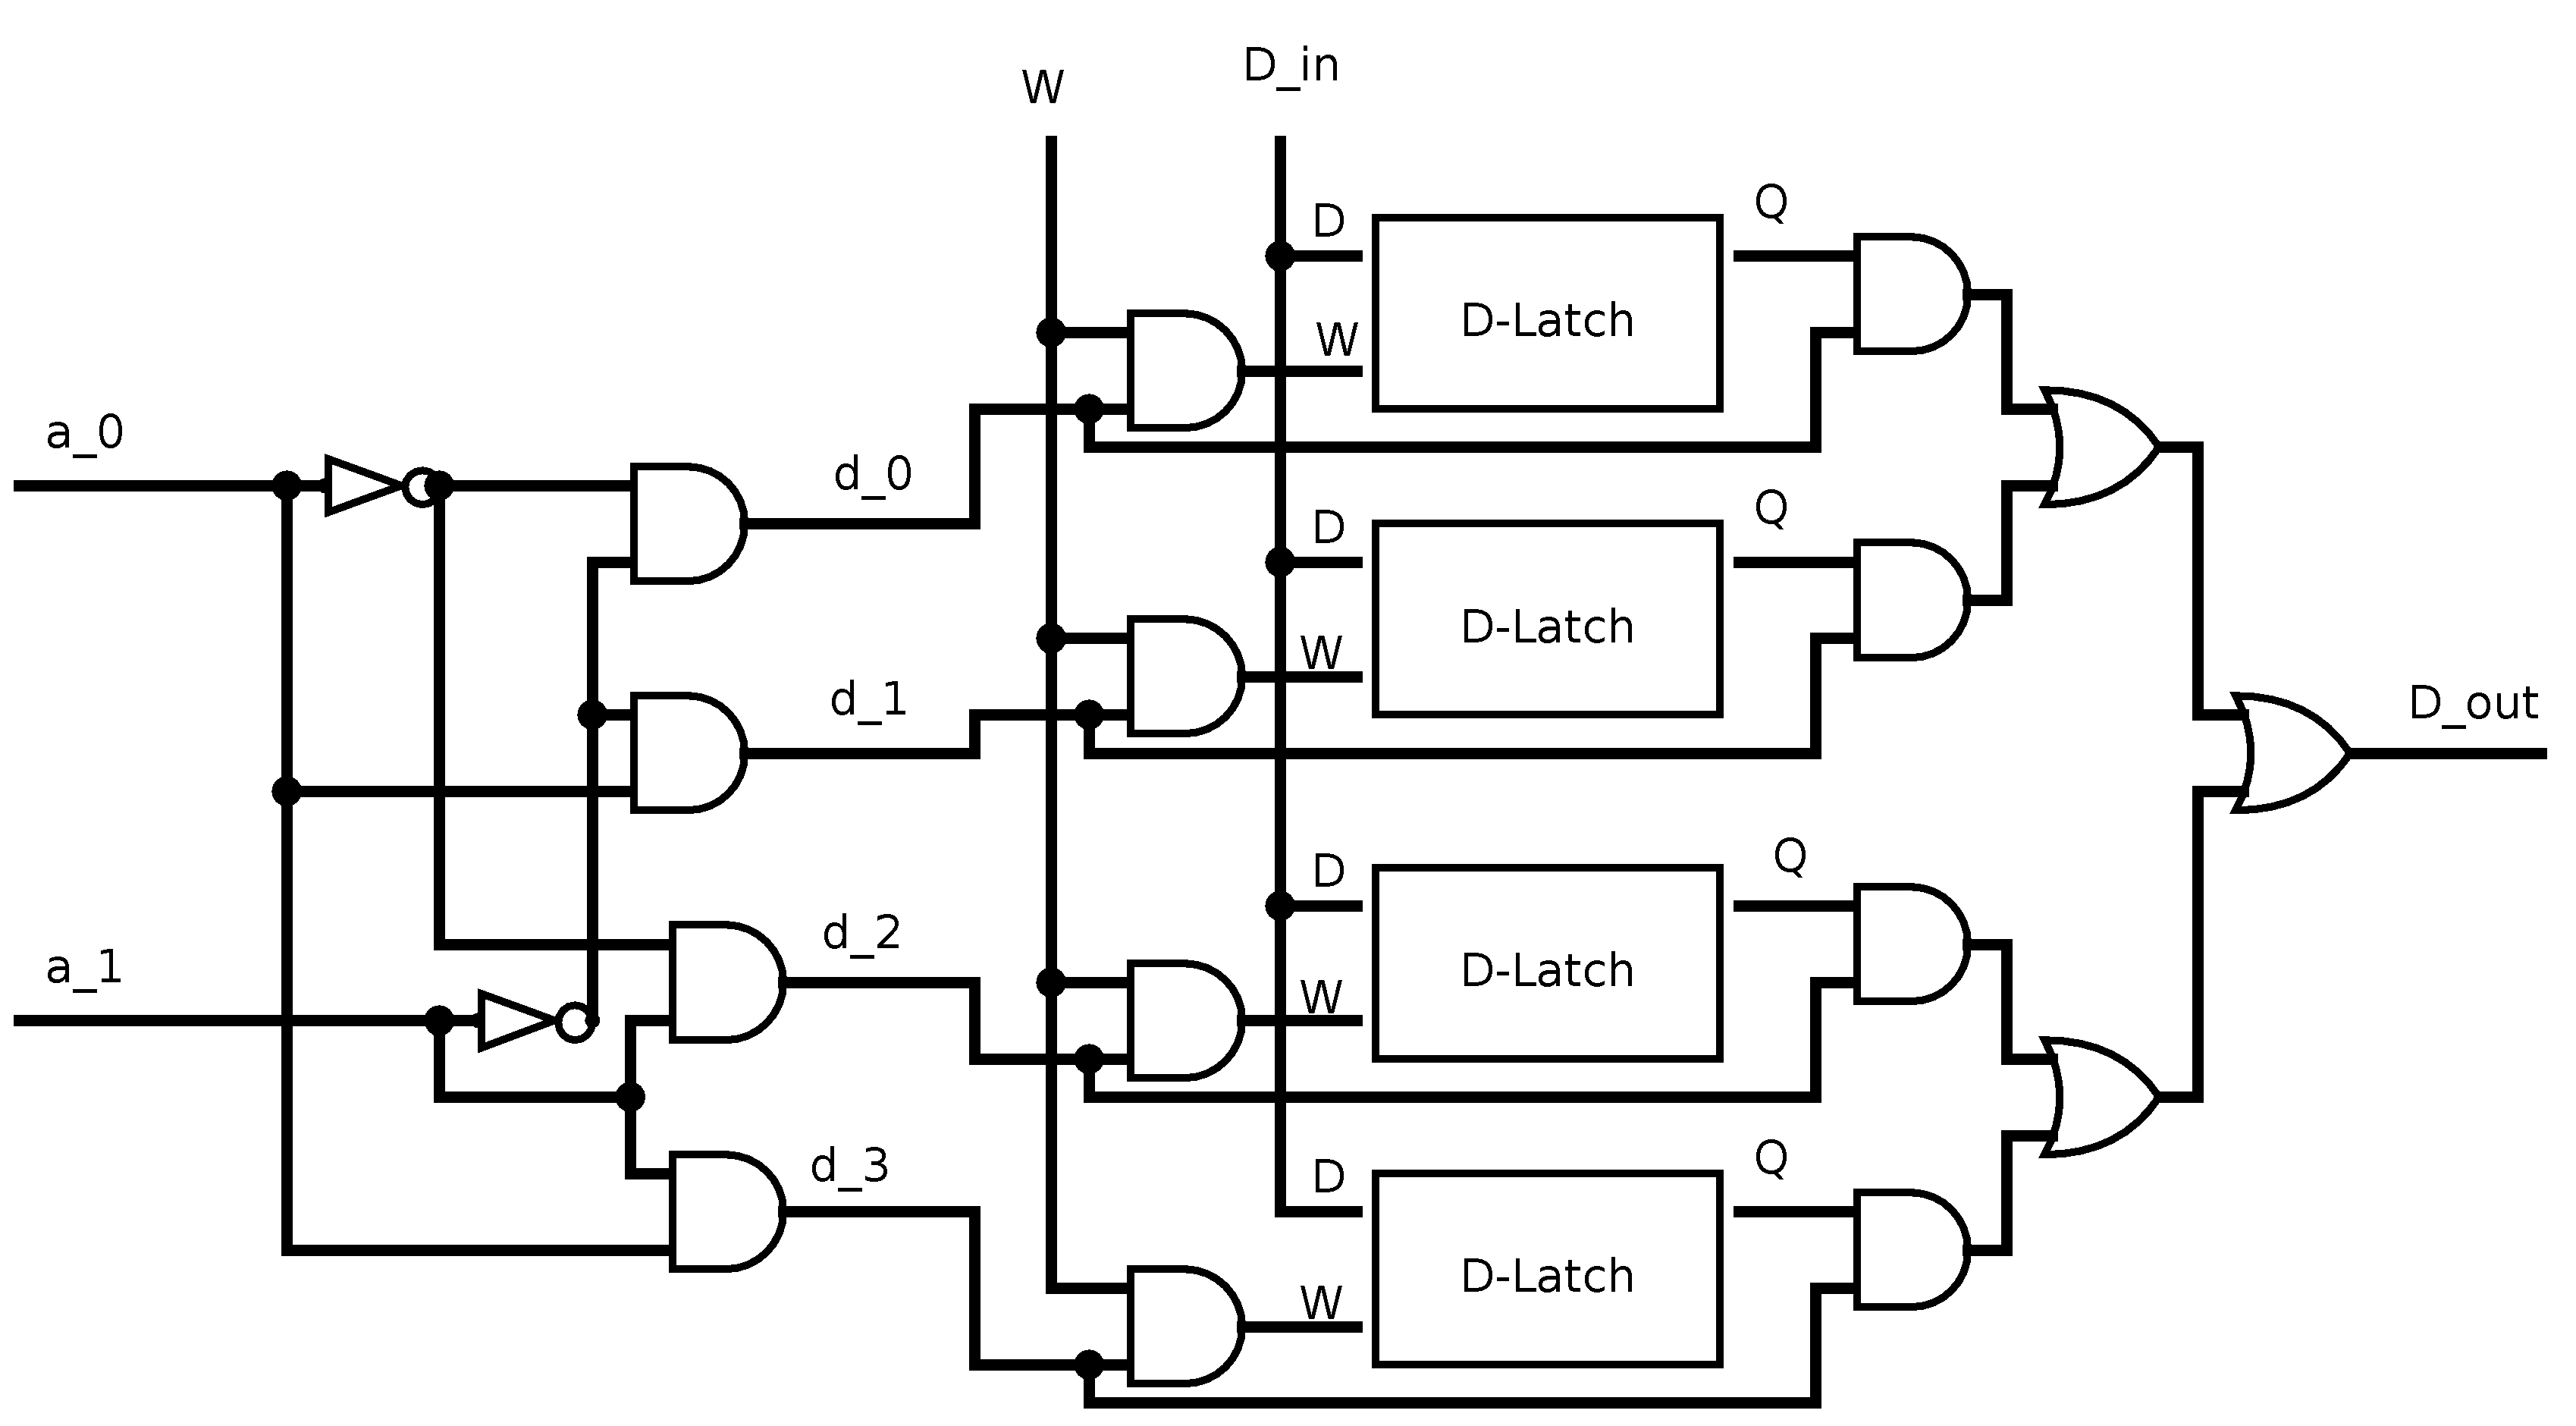
\includegraphics[width=14cm]{circuit_2.png}
    \item[c)] [Schaltkreis 3] \\
	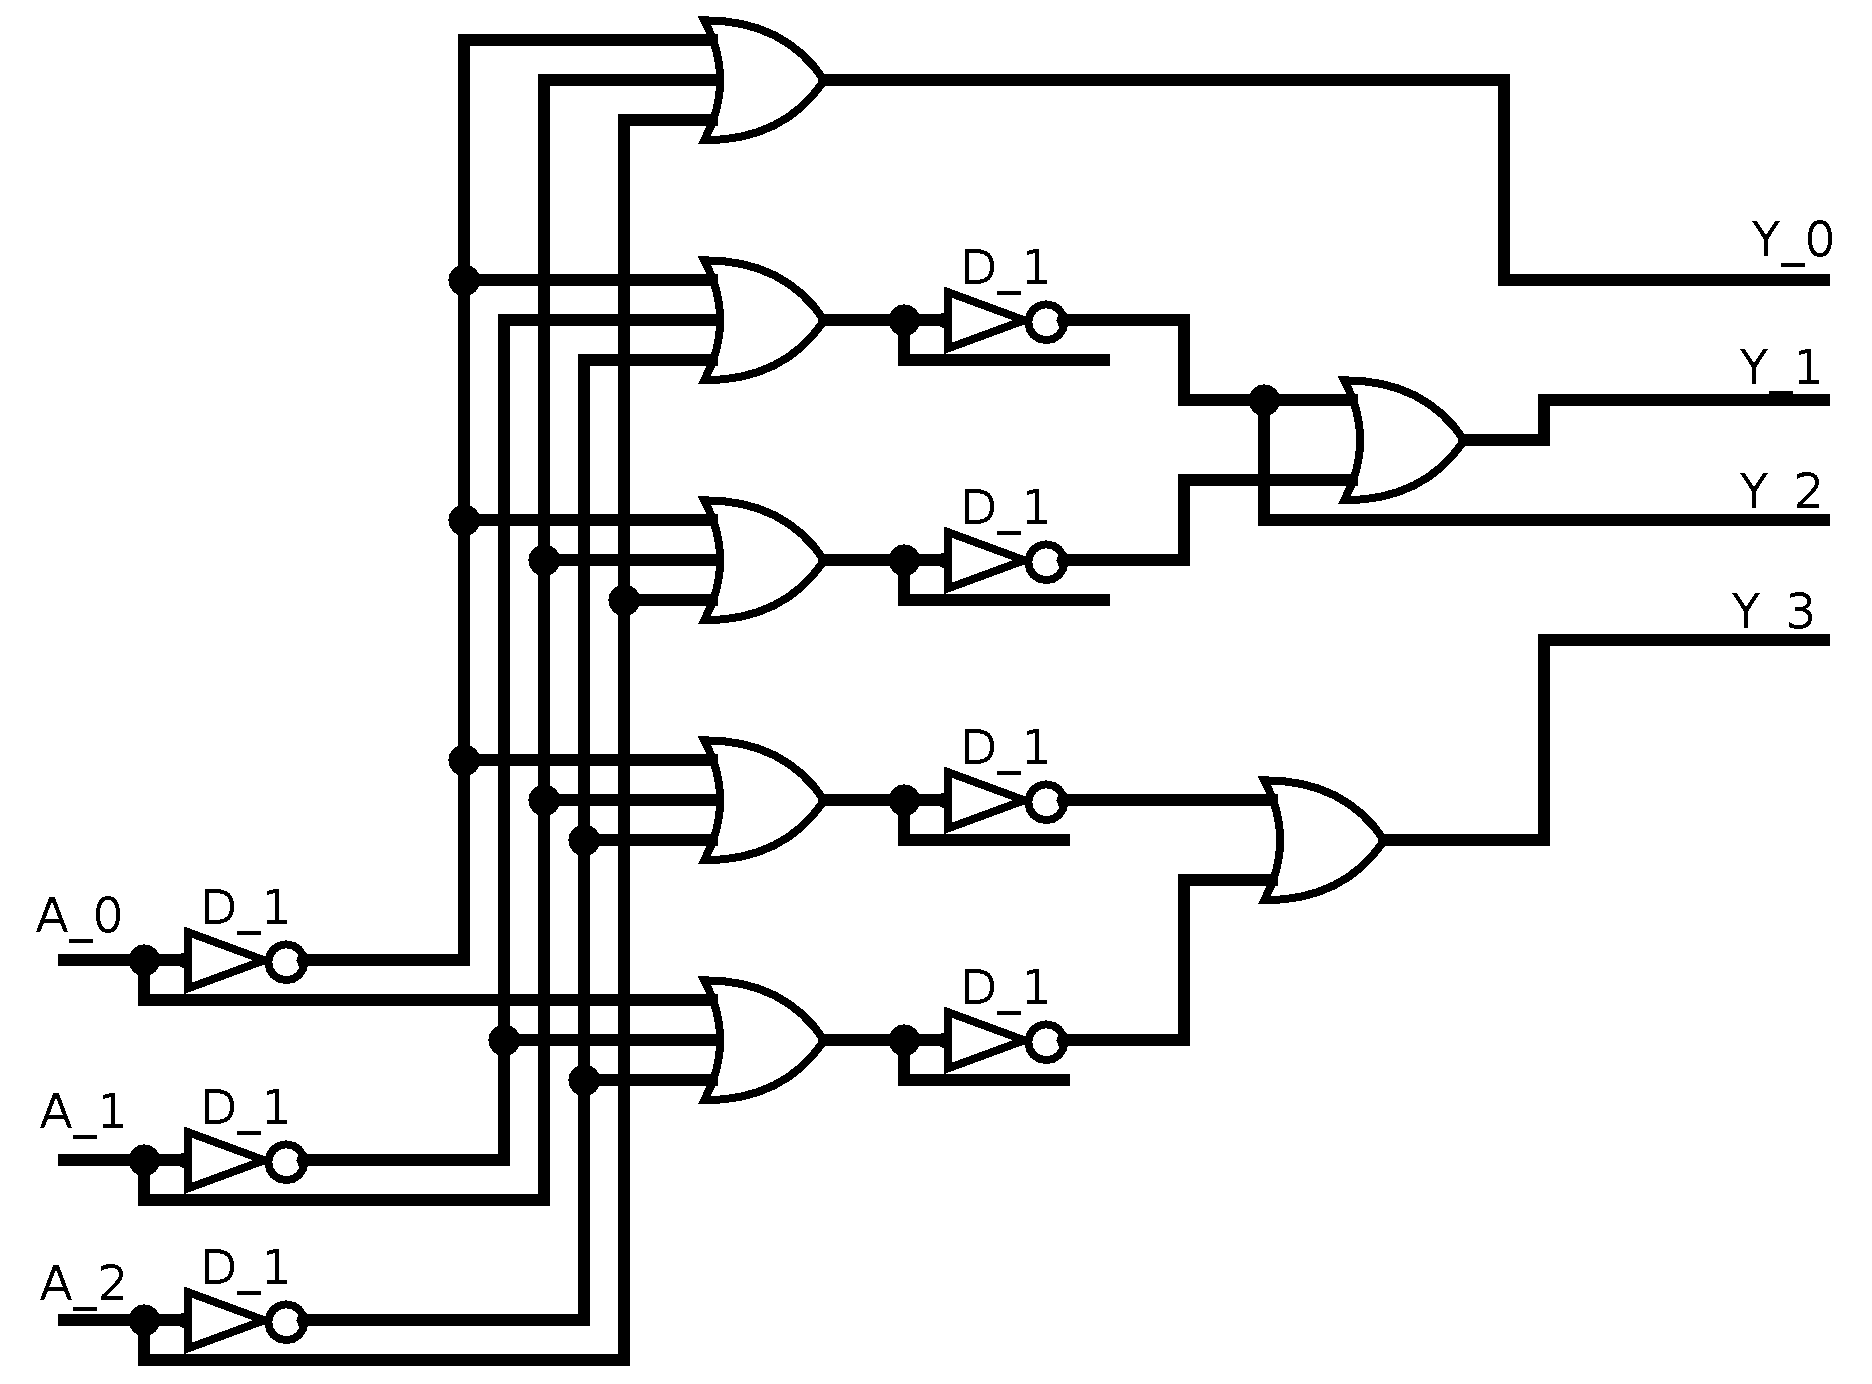
\includegraphics[width=14cm]{circuit_3.png}
        Datum: 12.11.1997, Funktion-ON-Mengen: \\
        $Y_0 = A_0' + A_1 + A_2$ \\
        $Y_1 = A_0A_1'A_2' + A_0A_1A_2$ \\
        $Y_2 = A_0A_1A_2$ \\
        $Y_3 = A_0A_1'A_2 + A_0'A_1A_2$ \\
        Begr�ndung: Da ein $D_1$-Dekoder 'zuf�llig' die Negation mit ausgibt, und \\
        $(B \wedge C) = \neg(\neg B \vee \neg C)$ ist, verwendet Diese Schaltung nur 'ODER'-Gatter und
        $D_1$-Dekoder.
\end{itemize}

\section*{Aufgabe 4}
\begin{itemize}

    \item Beh. $T(N)$ hat $N$ Bl�tter.
        Man nehme die Wurzel eines Baumes (z), ist $N = 1 (s = 0)$ sind wir fertig.
        Andernfalls nehmen wir unsere Wurzel als knoten und bekommen bis zu 10 weitere
        Teilb�ume. Ist $1 \leq N \leq 10$ nehmen wir $N$ entsprechend bl�tter und sind fertig,
        andernfalls nehmen wir jeweils $T(\lceil N/10 \rceil -1)$ als Teilb�ume. Unser Baum hat
        nun m�glicherweise mehr Bl�tter als gefordern ($N$), daher streichen wir die die zuviel
        sind zuf�llig weg. Und Voila, wir haben einen Baum $T(N)$ mit exakt $N$ Bl�ttern.

    \item Beh.: $T(N)$ hat $\leq N/9 + s$ innere Knoten. \\
        O.b.d.A.: $N \in \mathbb{N}$  (1,..) \\
        IA: $s = 0 \Leftrightarrow N \in \{10^{s-1} + 1,..., 10^s\} = N \in \{10^0 = 1\} = N = 1$.\\
        $T(1)$ hat $\leq N/9 + s = 1/9 + 0$ innere Knoten. Genauso: Pfadl�nge $s = 0$.
        Stimmt, da der Baum nur ein Blatt hat,
        das gleichzeitig die Wurzel ist. \\ \\
        IS: ($s \rightarrow s + 1$) \\
        Gilt f�r alle $N \in \{10^{s-1} + 1,..,10^s\} $.
        Wenn nun dieser Komplette Baum eine Ebene 'nach unten' verlegt wird, also die bisherige
        Wurzel nur noch Teilbaum der Neuen Wurzel ist, und neue Bl�tter erst auf der 'untersten'
        ebene hinzugef�gt werden (Ist dort kein platz mehr, werden neue 'pfade' von dem jew.
        niedrigsten noch nicht komplett ausgef�lltem Teilbaum auf diese ebene gebaut). \\
        Der Neue Baum hat dementsprechend pfadl�nge immer $s+1$ wenn der Bisherige Baum pfadl�nge
        $s$ gehabt hat (IV). \\
        Au�erdem hat er minimal $N/9 + s + 1$ innere Knoten (f�r $N = 10^s + 1$ )
        und maximal $(N/9) * 10 + s + 1$ (f�r $N = 10^{s+1}$), das sind $(10^s/9) * 10 + s + 1
        = 10^{s+1}/9 + (s + 1)$, also allgemein: \\
        Es gilt also: $T(N)$ hat $\leq N/9 + (s + 1)$ innere Knoten. \hfill $\Box$


\end{itemize}

\end{document}
